\chapter{Introduction and Motivation}


Autonomous sensing systems increasingly need to make spatial decisions at the edge: on small robots, wearable devices, and low-power platforms that cannot rely on continuous cloud computation. A fundamental spatial sensing problem is to estimate where an object is in three-dimensional space from a stream of physical measurements. In acoustic or radar-based systems, this means estimating range, horizontal angle (azimuth), and vertical angle (elevation) from reflected waves. The engineering challenge is not simply to make this estimate accurately in an ideal environment, but to do so under tight constraints on latency, memory, and power.


This project investigates a biomimetic approach to that problem. Instead of treating three-dimensional localisation as a generic black-box regression task, the model is built from functional analogues of the biological auditory system used by echolocating bats. Bats solve a closely related task with remarkable speed and efficiency. They emit short acoustic calls, receive returning echoes, and infer the three-dimensional structure of their environment in real time. The aim of this project is not to reproduce a bat brain in biophysical detail, but to identify the computational principles that make the biological solution attractive for engineered sensing.

The resulting system is a neuromorphic, bat-inspired model for active acoustic localisation. It emits a frequency-modulated call, simulates the returning binaural echo, converts the waveform into cochlear spike trains, processes distance, azimuth, and elevation through separate pathway models, and then combines the resulting population codes using continuous attractor readouts and a small trainable spiking network. The central question is whether a bottom-up, interpretable, pathway-based architecture can provide a useful alternative to an opaque end-to-end neural network.


\section{Neural Networks, Power, and Edge Devices}

Artificial neural networks (ANN) were originally modelled on their biological counterparts, with the neurons acting as logic gates \cite{Mcculloch1990AN}. There has been an increased focus on ANNs since the neural scaling laws discoveries instigated the age of artificial intelligence (AI) \cite{Kaplan2020ScalingModels}. However, with the increase in size and computational load of these multi-billion parameter models comes increased memory and power usage that is far exceeding the prediction of Moore's Law \cite{GholamiAIWall}. This not only has environmental consequences, but also constrains the use of these powerful neural networks for cloud computing in centralised data centres. The power requirements for neural networks are often too high for use on edge devices, such as autonomous cars, drones, or any other decentralised device. This creates a trade-off between the speed of on-device computing and the computational power that has to be pulled from an off-location data centre.

This project investigates a possible solution to low-power neural network use on edge devices, drawing inspiration from the original low-power edge devices that inspired neural networks in the first place. Spiking neural networks (SNNs) are a type of neural network that utilises the proven low power, high compute abilities of biological neurons, such as those within the brain. 
These SNNs have three key advantages over conventional ANNs: spikes, sparsity, and static suppression \cite{Eshraghian2023TRAININGLEARNING}. We will discuss these further in the next section, but simply put, they transfer information in an efficient way, and only when new information is received.


\section{Problem Specification}


The localisation task considered in this report is to estimate the polar coordinate vector
\begin{equation}
    \mathbf{x} = (r, \theta, \psi),
\end{equation}
where $r$ is target distance, $\theta$ is azimuth, and $\psi$ is elevation. This could be considered as a state space model (SSM) problem, where the hidden variables are the polar coordinates of the object, and observations are obtained by sending a signal to reflect off the object. In this project, we consider acoustic sound waves as our signal of choice.

\begin{figure}[H]
    \centering
    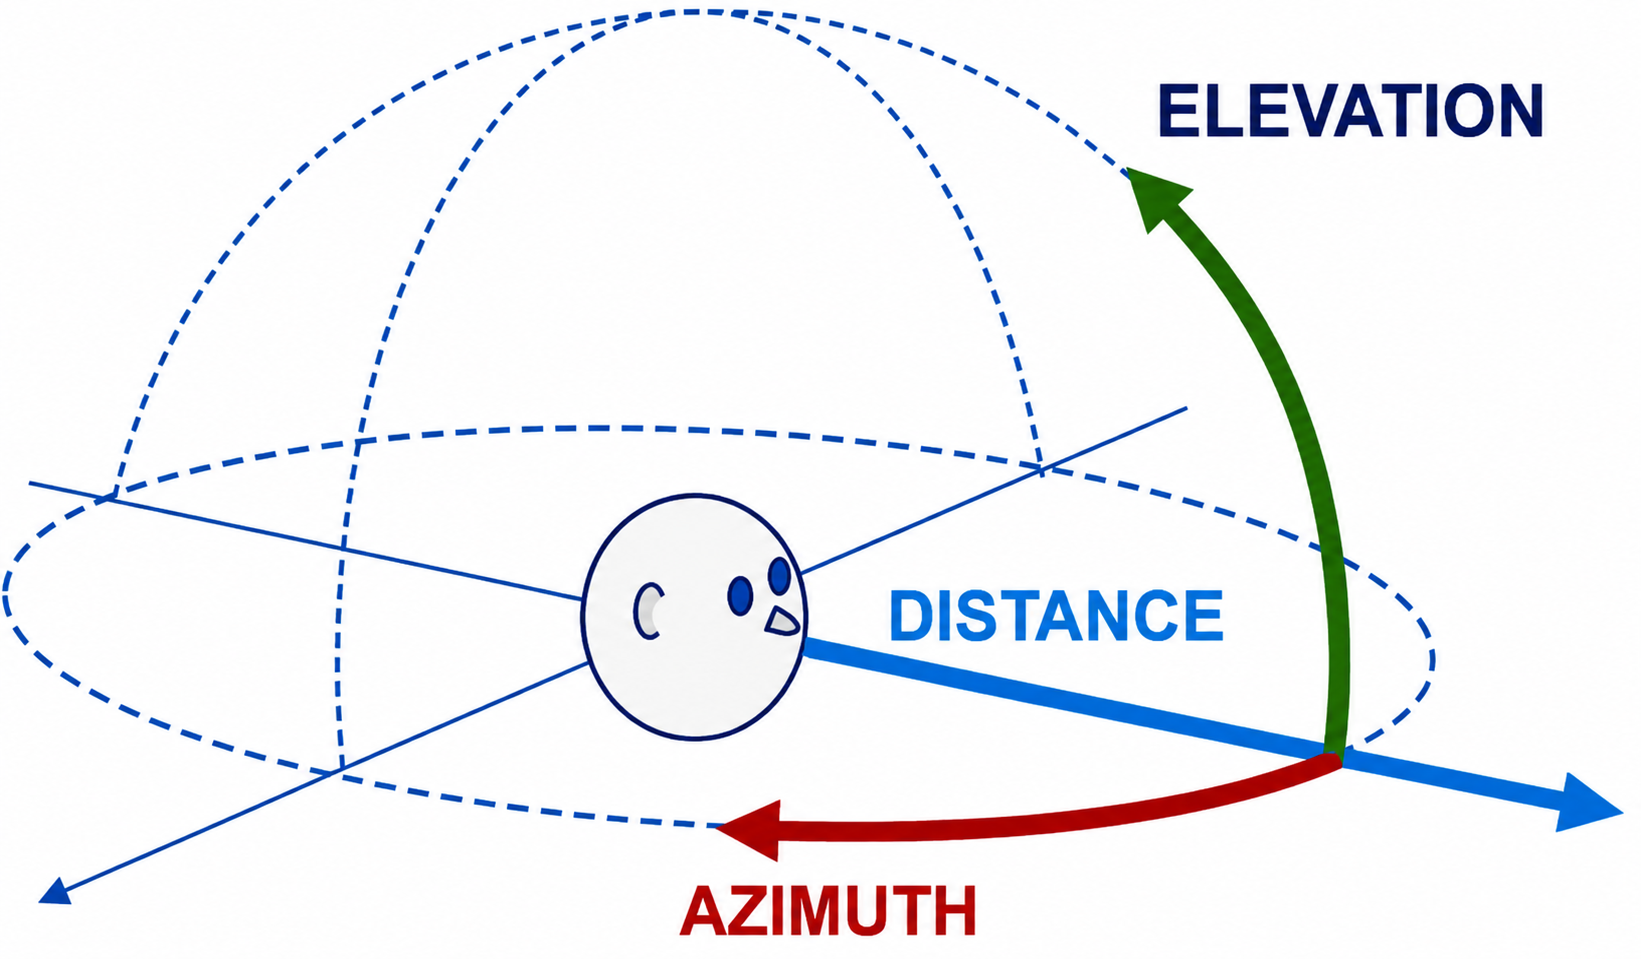
\includegraphics[width=0.72\linewidth]{1_Intro/intro_figures/polar_coords.png}
    \caption{Spherical coordinate representation of the localisation problem. The model estimates distance, azimuth, and elevation from the returning acoustic echo \cite{Carlini2024AuditoryReview}.}
    \label{fig:intro_spherical_coordinates}
\end{figure}

Conventional radar and sonar systems usually approach this problem through explicit signal processing. This is often multiple rounds of FFT with respect to different variables and consideration of constant false alarm rates (CFAR) in order to create a range-doppler map (RDM) (shown in figure \ref{fig:intro_radar}).  These methods are powerful and mathematically well understood. However, their reliance on dense numerical operations and constant processing makes them consume more power than is desirable.

\begin{figure}[H]
    \centering
    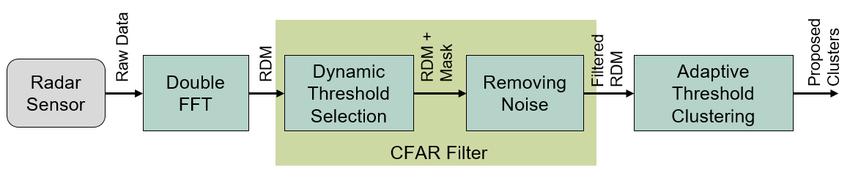
\includegraphics[width=0.72\linewidth]{1_Intro/intro_figures/radar_pipeline.png}
    \caption{Radar data processing pipeline with multiple heavy computation stages.}
    \label{fig:intro_radar}
\end{figure}

For large radars, high-performance sonars, or cloud-connected systems, this computational cost and power usage may be acceptable. For edge systems, it is more restrictive. A small autonomous device may need to localise targets while operating from a battery, with limited memory bandwidth and strict real-time latency. This shifts the design perspective from ``what is the most accurate algorithm?'', to ``what computations are worth the costs?''.


\section{Biomimetics and Echolocation}

Sensing the world around us is something that biological organisms do with relative ease. The complex structures that give organisms the ability to see and hear have evolved over hundreds of millions of years to create an intricate, finely tuned, detailed architecture that can process the surrounding environment. This makes biology the perfect blueprint to look for inspiration to develop more efficient neural networks. 

Biology provides a useful existence proof. Echolocating bats (or microchiroptera) solve a difficult active sensing problem using compact, low-power neural hardware. They estimate distance from echo delay, azimuth from binaural differences, and elevation from spectral shaping by their outer ear (or ``pinna''). They do this whilst flying, avoiding obstacles, and tracking prey in acoustically cluttered environments.

As an example comparison, current radar sensors for autonomous vehicles have a power consumption of 4.0-6.0 W, and are only used for lane change assistance, blind spot detection, and other simple functions \cite{Rajashekara2024DataReview}. On the other hand, bats have been measured to expend less than 1 W during echolocation, whilst also flying, breathing, and having basic metabolic functioning \cite{Speakman1989ThePipistrellus}. The echolocation of bats has also been hypothesised to create an auditory cognitive map which bats can use to navigate \cite{Krishna2025AuditoryHippocampus}, abilities far superior to the simple radar used for automatic braking on a car, and for less power use. The mechanisms of how biology achieves these feats are still not fully understood, however, this project aims to model some of the basic mechanisms to create a full end-to-end simulation of the brain of the bat.

\section{Aims and Objectives}


The overall aim of the project is to test whether a three-dimensional echolocation problem can be solved using a structured neuromorphic model inspired by the bat auditory system, rather than by an end-to-end black-box regressor. More specifically, the project asks whether biologically motivated pathways can provide useful intermediate representations for distance, azimuth, and elevation, and whether these representations can improve a small trainable SNN readout.

The main objectives are:
\begin{itemize}
    \item to construct a simulated active-acoustic environment in which an emitted FM call produces distance, azimuth, and elevation cues in the returning binaural echo;
    \item to develop a cochlear spike front end that converts the acoustic waveform into a tonotopic event-based representation suitable for downstream neuromorphic processing;
    \item to build separate distance, azimuth, and elevation pathways using simplified but interpretable biological computations, including delay coincidence, binaural comparison, and spectral-template matching;
    \item to investigate CANNs as SC-like population readouts, and to determine when attractor dynamics improve, stabilise, or distort the pathway populations;
    \item to compare direct pathway readouts, CANN readouts, calibrated readouts, and trainable SNN fusion in the same constrained localisation task;
    \item to test whether the pathway-derived feature set outperforms SNN baselines trained from less structured inputs such as raw binaural waveforms or cochlear spike rasters;
    \item to evaluate the final model under clean, environmental-noise, and reverberant conditions, while also identifying the limits of the constrained operating region.
\end{itemize}

The contribution of the project is therefore a complete modelling pipeline rather than a single isolated algorithm. The work shows how a complex active sensing task can be decomposed into interpretable neuromorphic components, how those components can be tested individually, and how a limited trainable readout can be added without discarding the biological structure. The final result supports a hybrid design principle: fixed biomimetic pathways are useful for feature extraction and interpretability, while a small trainable SNN is effective for contextual integration and residual correction.


\section{Report Structure}

Chapter 2 aims to provide the biological and signal-processing background needed to understand the model. It introduces auditory localisation cues, echolocation, spiking neurons, cochlear processing, and the major auditory pathways used as inspiration.

Chapter 3 describes the modelling and implementation. It explains the acoustic simulation, cochlear front end, distance pathway, azimuth pathway, elevation pathway, continuous attractor readouts, and trainable fusion network.

Chapter 4 presents the results. It evaluates the isolated pathways, the full fixed model, the effect of attractor readouts, the trainable residual readout, and the main runtime and scaling tradeoffs.

Chapter 5 concludes the report by summarising the main findings, discussing the limitations of the approach, and identifying future work needed to move from this prototype toward a more complete neuromorphic echolocation system.
